\section{Initial matching results}
\subsection{Vectortree matching}
When applying the vectortree matching algorithm to the candidate sets and target set, three sets of matchresults are generated. Table \ref{tab:results_from_vectortree} shows some examples of matches made by matching the birth certificates to the target set.

\afterpage{
	\clearpage
	\begin{landscape}
		\begin{table}
			\centering
			\caption[Example of vectortree output]{\label{tab:results_from_vectortree}Some matching results generated by the vectortree algorithm on birth certificates. The names of the groom and bride of the target registration are listed first. The names of the parents mentioned on the registration are listed in the last four columns. The Distance column indicates the edit distance over the two strings of all four names. }
				\resizebox{\columnwidth}{!} {
				\begin{tabular}{cc*4{l}c*4{l}}
					\toprule
					Distance & Target ID & Male first name & Male last name & Female first name & Female last name & Candidate ID & Male first name & Male last name & Female first name & Female last name \\
					\midrule
					2 & 701331 & cornelis & jansen & johanna & ee & 129230 & cornelis & jansen & janna & ee\\
					2 & 701331 & cornelis & jansen & johanna & ee & 161932 & cornelis & jansen & janna & ee\\
					0 & 704975 & francois & orlebeke & anna & ee & 92863 & francois & orlebeke & anna & ee\\
					0 & 704975 & francois & orlebeke & anna & ee & 347965 & francois & orlebeke & anna & ee\\
					0 & 704975 & francois & orlebeke & anna & ee & 373156 & francois & orlebeke & anna & ee\\
					0 & 704975 & francois & orlebeke & anna & ee & 439624 & francois & orlebeke & anna & ee\\
					0 & 704975 & francois & orlebeke & anna & ee & 480756 & francois & orlebeke & anna & ee\\
					0 & 704975 & francois & orlebeke & anna & ee & 524095 & francois & orlebeke & anna & ee\\
					2 & 891300 & jannis & verbrugge & johanna & ee & 71156 & jannis & verbrugge & janna & ee\\
					2 & 891300 & jannis & verbrugge & johanna & ee & 429783 & jannis & verbrugge & janna & ee\\
					1 & 811218 & jannis & reu & maria & eggel & 296559 & jannis & reu & maria & eggee \\
					\bottomrule
				\end{tabular}
			}
		\end{table}
	\end{landscape}
	\clearpage
}


Table \ref{tab:NumberOfMatches} shows the number of generated matches using the vector tree algorithm, per type of match and per maximum edit distance, as well as the number of extra matches that are generated when using a higher threshold compared to the number of matches with a threshold of 3. In total there are 130,277 extra matches with an edit distance of 4, and 317,287 extra matches with an edit distance of 5.\\
As expected, the number of matches increases strongly when increasing the threshold. 
 
 \begin{table}[ht]
 	\centering
 	\caption[Number of matches of vectortree per maximum edit distance]{The number of matches per maximum edit distance.\label{tab:NumberOfMatches}}
 	\begin{tabular}{llccclcccc}
 		\toprule
 		&& \multicolumn{3}{c}{Number of matches} && \multicolumn{4}{c}{Extra number of matches}\\
 		\cmidrule{3-5} \cmidrule{7-10}
 		Certificate type		&& th $\leq$ 3 & th $\leq$ 4 & th $\leq$ 5 && \multicolumn{2}{c}{th $\leq$ 4} & \multicolumn{2}{c}{th $\leq$ 5} \\
 		\cmidrule{1-1}\cmidrule{3-5} \cmidrule{7-10}	
 		marriage v.s. birth 	&& 556,549 & 610,645 & 741,555 && 54,096 & 109.72\% & 185,006 & 133.24\% \\
 		marriage v.s. marriage	&& 247,494 & 276,097 & 348,051 && 28,603 & 111.58\% & 100,557 & 140.63\% \\
 		marriage v.s. death 	&& 394,251 & 441,829 & 556,252 && 47,578 & 112.06\% & 162,001 & 141.09\% \\
 		\bottomrule\\
 		\multicolumn{5}{r}{Total extra matches:} && 130,277 & & 447,564 &\\
 		\bottomrule
 	\end{tabular}
 	
 \end{table}
 
Figure \ref{fig:dist_ed_per_th} shows the distribution of the error over the names. The edit distance per name pair is used as the labels for a match: if there are 4 names where the edit distance between the names on the target registration and the candidate registration is 1, the label `1,1,1,1' was assigned to that match, and if there is a match with an edit distance of 3 in a name and a name with an edit distance of 1, the label `1,3' is assigned to that match. The order in which the errors occur is not taken into account, as we treat an error in a first name the same as an error in a last name.\newline

The figure shows that a lot of matches have been generated where the error is concentrated in a single name. 55.9\% of all matches with a distance of 3 have the label 3, which means that the entire allowed error of 3 is concentrated in a single name. The same pattern can be seen for matches with an error of 4 and 5. 62.1\% of all matches with an error of 4 have a label of 4 and 46.1\% of all matches with an error of 5 have a label of 5.\\ 

In the vectortree matching, we assumed that all matches with an error of 3 can be accepted. Although an edit distance of 3 over the entire string seems as a sensible measure, these figures show that a lot of matches were generated where the error is concentrated in a single name. Since the average length of a name is between 6 and 7 characters, an error of 3 in a single name means that, on average, the names on the target and candidate registration differ in almost half of the number of characters. This suggests that the assumption that matches where the error is concentrated in a single name should be ignored when looking at higher edit distances is valid, while matches where the error is spread over multiple names can be considered as proper matches. 
\newline


Figure \ref{fig:dist_ed_per_name} shows the number of matches where the maximum distance is concentrated in a single name, broken down by the name type, for the set of matches where the candidate set is the set of marriage registrations of the children. This shows that increasing the threshold will primarily generate more matches in the family name, as discussed above and as indicated in chapter 3, since the number of matches where the error is concentrated in a single first name does not increase as much as the number of matches where the error is concentrated in the last name.


\begin{figure}
	\begin{center}
		\caption[Distribution of the maximum error over the names]{The distribution of the maximum allowed edit distance over the names for all the generated matches, grouped by error per name.}
		\centerline{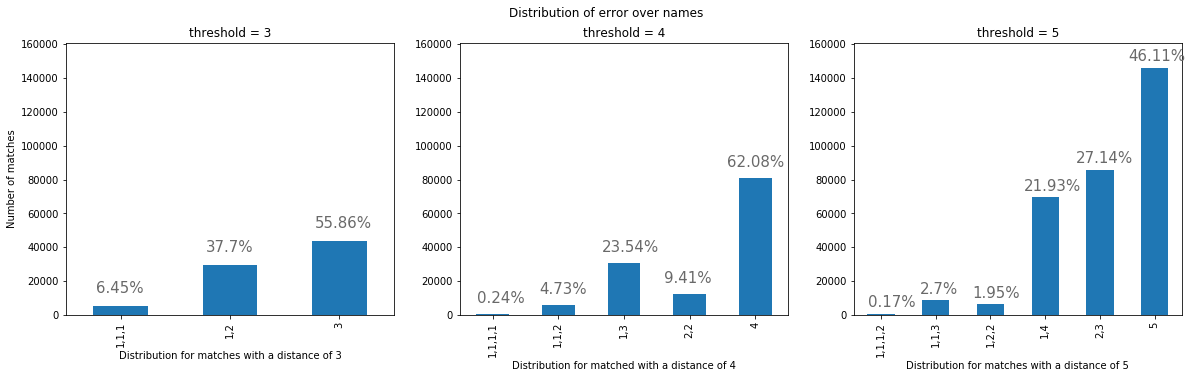
\includegraphics[scale=0.45]{figures/distribution_max_error_over_names_all.png}}
		\label{fig:dist_ed_per_th}
	\end{center}
	
\end{figure}

\begin{figure}
	\begin{center}
		\caption[Count max error per name]{Breakdown of the number of matches where the maximum allowed edit distance is concentrated in a single name for the matches generated on the marriage certificates.}
		\centerline{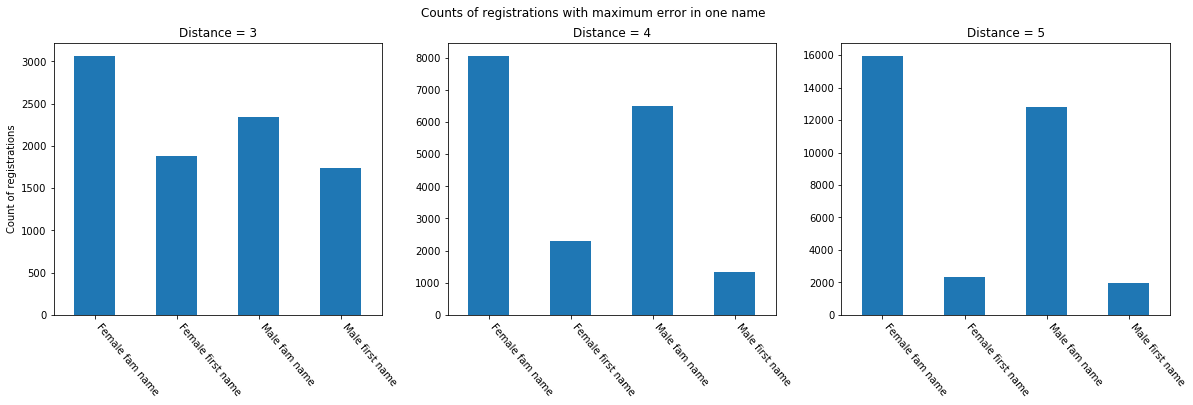
\includegraphics[scale=0.45]{figures/distribution_max_error_per_name_mar.png}}
		\label{fig:dist_ed_per_name}
	\end{center}
	
\end{figure}

\subsection{Overlinking and underlinking}

\begin{table}[ht]
	\centering
	\caption[Degree of overlinking per maximum edit distance]{The degree of overlinking per maximum edit distance. The overlinking is expressed as the number of parents linked per (unique) candidate certificate. The candidate certificates are the birth, marriage and death certificates of the children. \label{tab:OverlinkingMatches}}
	\vspace{0.25cm}
	\begin{tabular}{llccclccc}
		\toprule
		&& \multicolumn{3}{c}{Number of unique candidates} && \multicolumn{3}{c}{Average match per candidate}\\
		\cmidrule{3-5} \cmidrule{7-9}
		Certificate type		&& th $\leq$ 3 & th $\leq$ 4 & th $\leq$ 5 && th $\leq$ 3 & th $\leq$ 4 & th $\leq$ 5\\
		\cmidrule{1-1}\cmidrule{3-5} \cmidrule{7-9}	
		marriage v.s. birth 	&& 540,401 & 557,647 & 573,730 && 1.03 & 1.10 & 1.29\\
		marriage v.s. marriage	&& 142,414 & 147,218 & 154,033 && 1.74 & 1.88 & 2.26\\
		marriage v.s. death 	&& 390,960 & 401,082 & 422,082 && 1.01 & 1.10 & 1.32\\
	 	\bottomrule
	\end{tabular}
\end{table}
Table \ref{tab:OverlinkingMatches} shows the average number of matches generated per \textit{unique candidate} certificate. This is a measure on the overlinking results of the matching algorithm, as this table shows the (average) number of target certificate that each unique candidate certificate is matched to. For instance: with a threshold of 5, on average, each birth certificate is matched to 1.29 marriage certificate. To make this more concrete: on average, the matching algorthm found 1.29 pair of parents for each birth certificate when matching with a threshold of 5.\\

The average number of matches per candidate certificate for the birth- and death certificates for the matches with a maximum threshold of 3 is close to 1, which indicates that, on average, each candidate certificate is matched to a target certificate. This shows that, overall, the vectortree algorithm is able to match the candidate certificates very precisely to the target certificates for this type of certificates. \\

For marriage certificates, the expected average number of matches per candidate certificate should be around 2, as there are 2 pairs of parents present on each unique candidate certificate. However, the average number of matched target certificate is 1.74. This means that for these certificates there are actually matches missing, and the results from the vectortree algorithm show that there is a situation of underlinking. \\

As can be seen in table \ref{tab:NumberOfMatches} the vectortree algorithm generates 11\% more matches on marriages, when the threshold is increased to 4, but uses only 3.4\% more unique candidates (table \ref{tab:OverlinkingMatches}), and creates 41\% more matches when the threshold is increased to 5 and uses 8\% more unique candidates, compared to a threshold of 3. This shows that increasing the threshold will result in overlinking, as can be expected. This leads to an increase in the average number of match per unique candidate. Because this might not be a situation that is normally acceptable, we will filter out these results in the second and third phase.


\section{Named Pair based matching results}
In total, there are 556,549 matches on birth certificates with a Levenshtein distance of 3 or lower and 54,096 and 130,910 extra matches on Levenshtein distance 4 and 5, respectively. Ignoring the matches with a distance of 4 and 5 as described in section \ref{sec:name_pair_matching}, 20,681 matches remain with a distance of 4, and 34,952 matches remain with an edit distance of 5. \\
There are 247,494 matches for marriage certificates with an error of 3 or lower, and 28,603 and 71,954 matches with an error of 4 and 5, respectively. From the matches with an error of 4, we drop 18,201 matches as the error is concentrated in a single name. This results in 10,402 matches with an error of 4 that we accept. For the matches with error 5 we drop the matches with labels '5` and `2,3'. This means that we drop 52,645 matches and retain the remaining 19,226 matches.\\
Regarding the matches on the death certificates, we have 394,251 matches with a distance of 3 or smaller, 47,578 matches with an error of 4 and 114,423 matches with an error of 5. From the matches with edit distance 4 we drop 29,277 matches and retain 18,301 matches and from the matches with edit distance 5 we drop 83,808 matches and retain 30,615 matches. Table \ref{tab:breakdown_birth_matches} shows the breakdown of the matches that we have retained per label as well as the average number of matched target registrations per unique certificate. \\

The remaining matches with edit distance 4 and 5 are checked for compliance with the rules as described in table \ref{tab:Ruleset}. The acceptance rate for these matches is shown in table \ref{tab:acceptance_rate}. The acceptance rate, which is the ratio of matches that meet all the constraints as described in section \ref{sec:name_pair_matching}, is shown for matches where the additional prefix constraint is not applied (in the `Loose' column) and where the additional constraint is applied (in the `Strict' column). When comparing the acceptance rate for matches with edit distance 4 and 5, the matches with a distance of 5 are clearly less precise. This is expected, as the edit distance itself is a measure of certainty about the correspondence of two strings. Matches where the edit distance is distributed over more than two names seem to be more precise than matches where the error is concentrated on one or two names. This seems to support our assumption that matches with label `4', `1,4', `2,3' and `5' should not be accepted. \newline


\begin{table}
	\begin{center}
	\caption[Breakdown of all matches]{\label{tab:breakdown_birth_matches} A breakdown of matches per type of match. The labels represent the distribution of the error over the names of the matches. The average number of matches shows the degree of overlinking: the average number of target certificate (parent marriage certificates) that are linked to unique candidate certificates.}
	\vspace{0.5cm}
	\hspace*{-1.85cm}
	\resizebox{\columnwidth}{!} {
		\begin{tabular}{*{2}{crrr}crr}
			\toprule
			\multicolumn{11}{c}{Birth certificates}\\
			\toprule
			\multicolumn{3}{c}{Threshold: $\leq$3} & & \multicolumn{3}{c}{Threshold: 4} & & \multicolumn{3}{c}{Threshold: 5}\\
			Label & \# matches & avg. match & & Label & \# matches & avg. match & & Label & \# matches & avg. match \\
			\cmidrule{1-3} \cmidrule{5-7} \cmidrule{9-11} 
			0 		& 374,474 & 1.00 && 1,1,1,1 & 119 		& 1.01	&& 1,1,1,2 	& 224 		& 1.04\\
			1 		& 101,556 &	1.00 && 1,1,2   & 2,554		& 1.01 	&& 1,1,3 	& 3,546 	& 1.04\\
			1,1 	& 19,218  &	1.00 && 1,3 	& 12,821	& 1.05 	&& 1,2,2 	& 2,606  	& 1.03\\
			2 		& 27,656  &	1.00 && 2,2 	& 5,187		& 1.04 	&&  		&   		&\\
			1,1,1 	& 2,148   &	1.00 &&		   	&			&		&&			&			&\\
			1,2 	& 12,777  &	1.01 &&		   	&			&		&&			&			&\\
			3 		& 18,720  &	1.06 &&		   	&			&		&&			&			&\\
			\midrule
			Total: 	& 556,549 &	1.03 && 		& 20,681 	& 1.04	&&			& 6,376		& 1.04\\
			\bottomrule
		\end{tabular}
	}
		\hspace*{-1.85cm}

		\bigskip
	\resizebox{\columnwidth}{!} {
		\begin{tabular}{*{2}{crrr}crr}
			\toprule
			\multicolumn{11}{c}{Marriage certificates}\\
			\toprule
			\multicolumn{3}{c}{Threshold: $\leq$ 3} & & \multicolumn{3}{c}{Threshold: 4} && \multicolumn{3}{c}{Threshold: 5}\\
			Label & \# matches & avg. match & & Label & \# matches & avg. match & & Label & \# matches & avg. match \\
			\cmidrule{1-3} \cmidrule{5-7} \cmidrule{9-11} 
			0 		& 166,849 &	1.47 && 1,1,1,1	& 61	 & 1.00	&& 1,1,1,2 	& 111   	& 1.00\\
			1 		& 44,785  &	1.10 && 1,1,2 	& 1,221  & 1.03	&& 1,1,3 	& 1,907 	& 1.04\\
			1,1 	& 8,234   &	1.03 && 1,3 	& 6,538  & 1.07	&& 1,2,2 	& 1,351 	& 1.03\\
			2 		& 12,027  &	1.03 && 2,2 	& 2,582  & 1.05	&& 			&			&\\
			1,1,1 	& 980     &	1.01 &&			&		 &	&&				&			&\\
			1,2 	& 5,608   &	1.03 &&			&		 &	&&				&			&\\
			3 		& 9,011   &	1.08 &&			&		 &	&&				&			&\\
			\midrule
			Total: 	& 247,494 &	1.74 && 		& 10,402 & 1.06	&&			& 3,369 	& 1.04\\
			\bottomrule
		\end{tabular}
	}
		\hspace*{-1.85cm}

		\bigskip
	\resizebox{\columnwidth}{!} {
		\begin{tabular}{*{2}{crrr}crr}
			\toprule
			\multicolumn{11}{c}{Death certificates}\\
			\toprule
			\multicolumn{3}{c}{Threshold: $\leq$ 3} & & \multicolumn{3}{c}{Threshold: 4} && \multicolumn{3}{c}{Threshold: 5}\\
			Label & \# matches & avg. match & & Label & \# matches & avg. match & & Label & \# matches & avg. match \\
			\cmidrule{1-3} \cmidrule{5-7} \cmidrule{9-11} 
			0 		& 246,288 & 1.00	&& 1,1,1,1 	& 135	 & 1.02	&& 1,1,1,2 	&  202	  & 1.03\\
			1 		& 80,103  &	1.00	&& 1,1,2 	& 2,387  & 1.01	&& 1,1,3 	&  3,106  & 1.03\\
			1,1 	& 16,209  &	1.00	&& 1,3 		& 11,297 & 1.05	&& 1,2,2 	&  2,229  & 1.03\\
			2 		& 22,743  &	1.00	&& 2,2 		& 4,482  & 1.03	&&   		&   	  & \\
			1,1,1 	& 1,910   &	1.00 	&&			&			&&			&&\\
			1,2 	& 11,007  &	1.00 	&&			&			&&			&&\\
			3 		& 15,921  &	1.05	&&			&			&&			&&\\
			\midrule
			Total: 	& 394,181 &	1.01 	&& 			& 18,301 & 1.04	&&			& 5,537   & 1.03\\
			\bottomrule
		\end{tabular}
	}
	\hspace*{-1.85cm}
	\end{center}
\end{table}



\begin{table}
	\begin{center}
		\caption[Acceptance rate]{\label{tab:acceptance_rate} The acceptance rates for edit distance 4 and 5 on the ruleset in table \ref{tab:Ruleset}. The acceptance rate describes the percentage of generated matches per label that comply with these rules. The 'Loose' columns show the acceptance rate of matches when the constraint on matching starting characters is not applied, whereas the 'Strict' columns show the rates where this constraint is applied. }
		\vspace{0.5cm}
		\resizebox{\columnwidth}{!} {
			\begin{tabular}{*{13}{c}}
				\toprule
				\multicolumn{13}{c}{Acceptance rate - Birth $\leftrightarrow$ Marriage  certificates}\\
				\midrule
				\multicolumn{6}{c}{Threshold: 4} && \multicolumn{6}{c}{Threshold: 5}\\
				\cmidrule{1-6} \cmidrule{8-13}
				Label 	& \# matches & \multicolumn{2}{c}{Loose}	& \multicolumn{2}{c}{Strict} && Label 	& \# matches & \multicolumn{2}{c}{Loose}	& \multicolumn{2}{c}{Strict} \\
				\cmidrule{1-2} \cmidrule{3-4} \cmidrule{5-6} \cmidrule{8-13} 
				1,1,1,1 & 119 		& 43.70\% & 52 		& 31.09\% 	& 37 	&& 1,1,1,2 	& 224		& 50.00\% 	& 112	& 33.03\% & 74	\\
				1,1,2 	& 2,554 	& 59.71\% & 1,525 	& 35.83\% 	& 915 	&& 1,1,3 	& 3,546		& 36.91\% 	& 1,309	& 15.48\% &	549 \\
				1,3 	& 12,821 	& 47.35\% & 6,071 	& 18.48\% 	& 2,369	&& 1,2,2 	& 2,606		& 35.03\%	& 913 	& 12.70\% & 331 \\
				2,2 	& 5,187 	& 47.27\% & 2,452 	& 17.27\% 	& 896	&&  		& 	&   	& 	&   &  \\
				\midrule
						& 20,681	& 48.84\% & 10,100 	& 20.39\%	& 4,217	&&			& 6,376	& 36.6\%	& 2,334 & 14.96\% & 954\\
				\bottomrule
			\end{tabular}
		}
		\bigskip
		
		\resizebox{\columnwidth}{!} {
			\begin{tabular}{*{13}{c}}
				\toprule
				\multicolumn{13}{c}{Acceptance rate - Marriage $\leftrightarrow$ Marriage certificates }\\
				\midrule
				\multicolumn{6}{c}{Threshold: 4} && \multicolumn{6}{c}{Threshold: 5}\\
				\cmidrule{1-6} \cmidrule{8-13}
				Label 	& \# matches & \multicolumn{2}{c}{Loose}	& \multicolumn{2}{c}{Strict} && Label 	& \# matches & \multicolumn{2}{c}{Loose}	& \multicolumn{2}{c}{Strict} \\
				\cmidrule{1-2} \cmidrule{3-4} \cmidrule{5-6} \cmidrule{8-13} 
				1,1,1,1 & 61 		& 32.78\% & 20 		& 18.03\% & 11 		&& 1,1,1,2 	& 111		& 44.14\% & 49		& 31.53\% & 35\\
				1,1,2 	& 1,221		& 58.23\% & 711		& 34.46\% & 422		&& 1,1,3 	& 1,907		& 33.67\% & 642		& 15.21\% & 290\\
				1,3 	& 6,538		& 43.27\% & 2,829	& 16.20\% & 1,059	&& 1,2,2 	& 1,351		& 33.46\% & 452		& 12.06\% & 163\\
				2,2 	& 2,582		& 42.72\% & 1,103	& 12.59\% & 325		&&  		& 			&  	 & 	&  & \\
				\midrule
						& 10,402	& 44.83\% & 4,667 	& 17.48\% & 1,817	&&			& 3,369		& 34.22\% & 1,153 	& 14.49\% & 488\\
				\bottomrule
			\end{tabular}
		}

		\bigskip

		\resizebox{\columnwidth}{!} {
			\begin{tabular}{*{13}{c}}
				\toprule
				\multicolumn{13}{c}{Acceptance rate - Death $\leftrightarrow$ Marriage certificates}\\
				\midrule
				\multicolumn{6}{c}{Threshold: 4} && \multicolumn{6}{c}{Threshold: 5}\\
				\cmidrule{1-6} \cmidrule{8-13}
				Label 	& \# matches & \multicolumn{2}{c}{Loose}	& \multicolumn{2}{c}{Strict} && Label 	& \# matches & \multicolumn{2}{c}{Loose}	& \multicolumn{2}{c}{Strict} \\
				\cmidrule{1-2} \cmidrule{3-4} \cmidrule{5-6} \cmidrule{8-13} 
				1,1,1,1	& 135 		& 43.70\% & 59 		& 28.89\%	& 39	&& 1,1,1,2 & 202	& 49.00\% & 99 		& 31.68\% & 64	\\
				1,1,2 	& 2,387		& 60.20\% & 1,437	& 36.57\%	& 873	&& 1,1,3   & 3,106	& 37.54\% & 1,116	& 17.58\% & 546	\\
				1,3 	& 11,297	& 47.48\% & 5,364	& 18.74\%	& 2,117	&& 1,2,2   & 2,229	& 34.99\% & 780		& 14.09\% &	314	\\
				2,2 	& 4,482		& 46.63\% & 2,090	& 16.17\%	& 725	&&   & &   & 	&   & 	\\
				\midrule
						& 18,301	& 48.96\% & 8,961 	& 20.51\%	& 3,754	&&		   & 5,537 & 36.03\% &  1,995	& 16.69\%  & 924\\
				\bottomrule
			\end{tabular}
		}
	\end{center}
\end{table}



\section{Filtering birth certificates}

\begin{figure}
	\begin{center}
		\caption[Consistency check acceptance rate (no prefix constraint)]{\label{fig:consistency_check_loose}Percentage of rejected and accepted matches by the extra checks on consistency. The matches that are checked are the matches that are accepted when name pair based matching is performed without the extra constraint on the matching prefixes. (Loose) }
		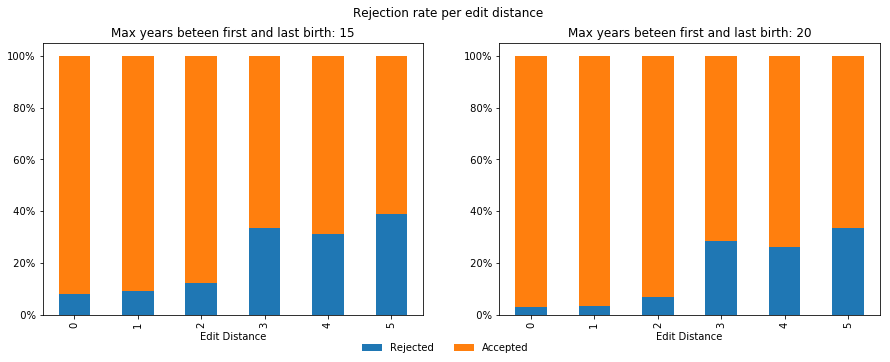
\includegraphics[scale=0.45]{figures/rejection_rate_loose.png}
		\caption[Consistency check acceptance rate (with prefix constraint)]{\label{fig:consistency_check_strict} Percentage of rejected and accepted matches by the extra checks on consistency. These matches are the matches that are accepted when name pair based matching is performed with the extra constraint on matching prefixes. (Strict)}
		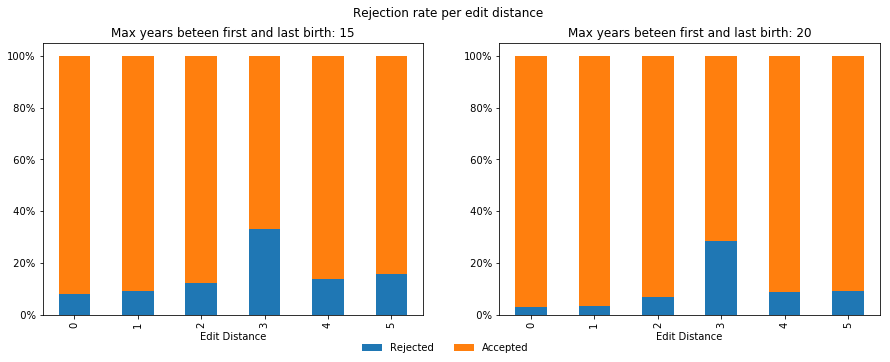
\includegraphics[scale=0.45]{figures/rejection_rate_strict.png}
		\vspace{0.5cm}
	\end{center}
\end{figure}

The matches on birth certificates that are accepted as described in the previous section are checked for consistency. Figures \ref{fig:consistency_check_strict} and \ref{fig:consistency_check_loose} show the percentages of accepted and rejected matches for the matches with and without the additional matching starting characters constraint, respectively. The name pair matching constraints are only checked for matches with Levenshtein distance 4 and 5.\\
The left plot in both figures shows the number of rejected and accepted matches when the maximum number of years between the first and last birth match is 15 at most, and the right plot shows the same percentages, but when the maximum number of years is 20. In both figures, the number of accepted matches is higher when the maximum allowed years is 20 years. This is expected, as this requirement is less restrictive on the matches. \\

Since matches with a distance of 3 where assumed to be correct matches it is of interest to note that the number of rejected matches increases significantly at edit distance 3. Table \ref{tab:rejection_rate_label} shows that this is mainly contributed by the matches where the distance is concentrated in a single name. Although the majority is accepted by our consistency checks, the rise of the rejection rate suggests that the assumption - that matches with edit distance 3 are safe to accept - must be adjusted and that matches with a distance of 3 in a single name should be investigated further. \\
The effect of additional constraints on matches is clearly visible in the matches with edit distance 4 and 5. With no additional constraint on the prefix, the rejection rate of these matches is around 35\% to 40\% for matches with a maximum of 15 year between the first and last birth certificate. With the additional prefix constraint, the rejection rate drop to between 15\% and 20\%. \\

Table \ref{tab:rejection_rate_label} shows the rejection rate per label. The rejection rate of matches without the additional prefix constraint is lowest when the distance is distributed over all names (or over three in case of a distance of 3), like we expected, and increases as the error is more concentrated in one name, as seen in the previous section. The rejection rate for the matches that comply with the extra prefix constraint seems to be evenly distributed. This is further evidence that the constraint on the prefix of the names can be used in order to distinguish matches when there is a larger distance between the names.


\begin{table}
	\begin{center}
		\caption[Rejection rate per label]{\label{tab:rejection_rate_label}The rejection rate per label shows that the additional prefix constraint filters out a large chunk of the inconsistent matches generated with edit distance 4 and 5 on matches where the maximum difference between the first and last birth certificate in a family is 15 years.}
		\vspace{0.5cm}
	\begin{tabular}{*{4}{l}}
		\toprule
		Distance & Label & Loose & Strict \\
		\toprule
		\multirow{3}{*}{3} & 1,1,1 & 0.057 & 0.057 \\
		& 1,2 & 0.132 & 0.132 \\
		& 3 & 0.433 & 0.433 \\
		\midrule
		\multirow{4}{*}{4} & 1,1,1,1 & 0.115 & 0.162 \\
		& 1,1,2 & 0.087 & 0.079 \\
		& 1,3 & 0.281 & 0.084 \\
		\midrule
		\multirow{4}{*}{5} & 1,1,1,2 & 0.116 & 0.135 \\
		& 1,1,3 & 0.256 & 0.082 \\
		& 1,2,2 & 0.383 & 0.121 \\
		\bottomrule
	\end{tabular}
	\end{center}
\end{table}

\section{Discussion}
Since we do not have a set of matches that we know are correct, it is impossible to compute objective measures of performance for the matching results. However, it is possible to evaluate the performance of the matches on the rule set introduced in the third step of the matching process.\\ 

The distribution of the error over the names for matches with an error of 3 showed that for 55.9\% of these matches the error was concentrated in a single name. This suggest that the assumption that matches with an edit distance of 3 over the entire string of four names are acceptable might be reevaluated, or that the results with an edit distance of 3 should be tested further. The threshold of 3 seems sensible if the error is distributed over all four names. When the error is concentrated in a single name the rejection rate of the consistency check increases, and therefore further analysis is needed for matches with an edit distance of 3.\\

When increasing the threshold for the initial matching algorithm to 4 or 5 in order to be more lenient towards spelling variantions, a lot of extra matches will be generated. As with the matches with an error of 3, care should be taken to accept these extra matches. The vast majority of extra matches will be generated by matches where there is a distance of 3 in a single name. 
When choosing to filter these extra matches on name pairs, the rules as desribed in table \ref{tab:Ruleset} can be used to filter out these unwanted matches. We have tested the ruleset on matches with a maximum edit distance of 4 and 5. The ruleset seems to perform well on both the matches made with distance 4 and 5, as the rejection rate of the matches with these distances that are accepted by this ruleset in the second step of the procedure, and accepted by the consistency checks in the third step of the procedure does not increase significantly when matched with distance 5, compared to matches with distance 4.\\

As can be seen in table \ref{tab:acceptance_rate}, the rules in the second step can filter out a great deal of extra generated matches and are effective in filtering matches that are made with a large distance concentrated in a single name.\\

As mentioned before, there is no way to be certain that the generated matches are actually correct. It is therefore difficult to assess the effectiveness and performance of the approach in this thesis in a coherent, objective way. However, when using edit distance, one can be fairly certain that, with a low edit distance and if consistent with domain knowledge, these matches are indeed proper matches. Whenever the edit distance increases, the matches that are made with a more distributed error are more safe to accept than matches where the error is concentrated in fewer names.